%\usetikzlibrary{positioning}
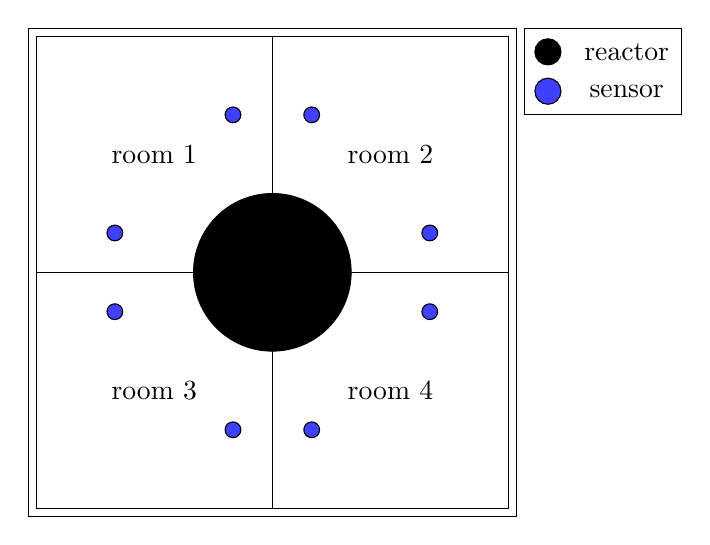
\begin{tikzpicture}
%shielding
\draw (-.1,-.1) rectangle (6.1,6.1);
%reactor
\draw[fill] (3,3) circle (1);
\node[draw,circle,fill] (reactor-icon) at (6.5,5.8) {};
\node (reactor) [right of = reactor-icon] {reactor};

%room 1
\draw (0,3) rectangle (3,6);
\node (room1) at (1.5,4.5) {room 1};
\draw[fill=blue!75] (2.5,5) circle (.1);
\draw[fill=blue!75] (1,3.5) circle (.1);
%room 2
\draw (0,0) rectangle (3,3);
\node (room1) at (4.5,4.5) {room 2};
\draw[fill=blue!75] (3.5,5) circle (.1);
\draw[fill=blue!75] (5,3.5) circle (.1);
%room 3
\draw (3,3) rectangle (6,6);
\node (room1) at (1.5,1.5) {room 3};
\draw[fill=blue!75] (2.5,1) circle (.1);
\draw[fill=blue!75] (1,2.5) circle (.1);
%room 4
\draw[fill=blue!75] (3.5,1) circle (.1);
\draw[fill=blue!75] (5,2.5) circle (.1);
\draw (3,0) rectangle (6,3);
\node (room1) at (4.5,1.5) {room 4};

%legend
\node[draw,circle,fill=blue!75] (sensor-icon) at (6.5,5.3) {};
\node (reactor) [right of = sensor-icon] {sensor};

%legend-border
\draw (6.2,5) rectangle (8.2,6.1);
\end{tikzpicture}